\documentclass[11pt,oneside]{book}

\usepackage[T1]{fontenc}
\usepackage[margin=1in]{geometry}
\usepackage{graphicx}
\usepackage[hidelinks]{hyperref}
\usepackage{xcolor}
\usepackage{listings}

\definecolor{codebackground}{RGB}{245,247,250}
\definecolor{codeframe}{RGB}{205,211,220}
\definecolor{coverpaper}{RGB}{248,221,186}
\definecolor{coverink}{RGB}{35,54,61}

\lstset{
  basicstyle=\ttfamily\small,
  backgroundcolor=\color{codebackground},
  frame=single,
  rulecolor=\color{codeframe},
  columns=fullflexible,
  keepspaces=true,
  showstringspaces=false
}

\title{Rails on Jails\\[0.5em]\large End-to-End Testing on FreeBSD}
\author{The BSDRunner Project}
\date{\today}

\begin{document}

\frontmatter
\hypersetup{pageanchor=false}
\begin{titlepage}
  \pagecolor{coverpaper}
  \color{coverink}
  \centering
  \vspace*{0.35in}

  {\fontsize{35.83}{42}\selectfont\bfseries Rails on Jails\par}
  \vspace{0.25em}
  {\Large End-to-End Testing on FreeBSD\par}
  \vspace{0.3in}

  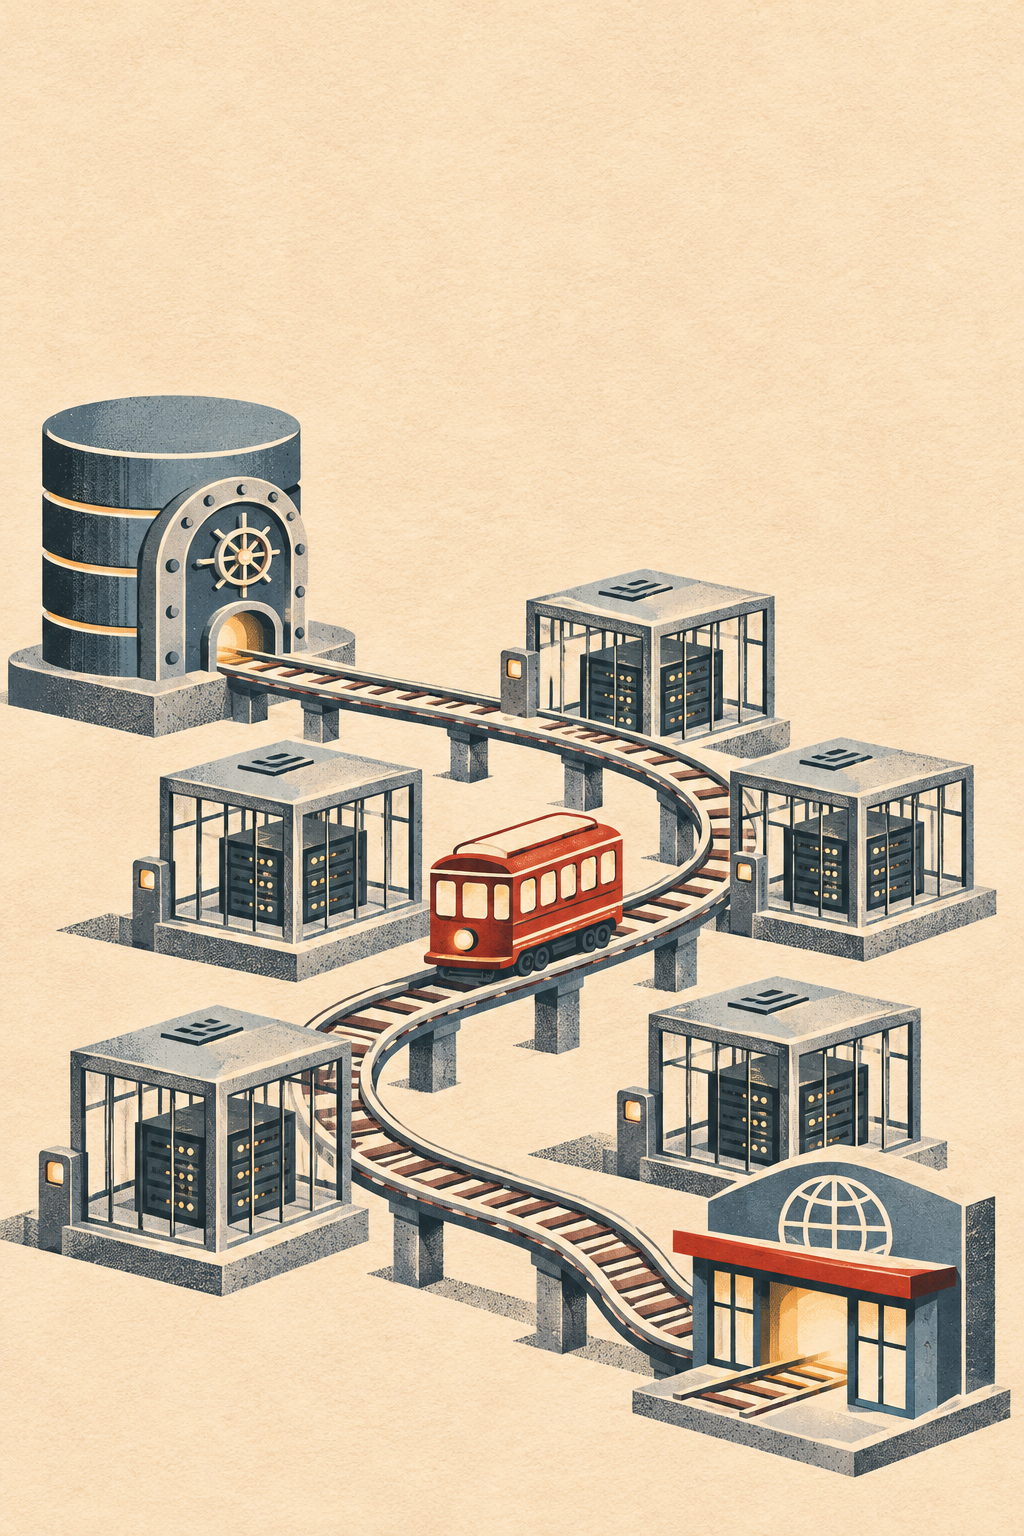
\includegraphics[
    width=0.92\textwidth,
    height=0.66\textheight,
    keepaspectratio,
    trim=0 0 0 340,
    clip
  ]{assets/rails-on-jails-cover.png}

  \vfill
  {\large The BSDRunner Project\par}
  \vspace{0.35em}
  {\normalsize \today\par}
\end{titlepage}
\nopagecolor
\color{black}
\hypersetup{pageanchor=true}
\tableofcontents

\mainmatter
\chapter{A Small System with Real Boundaries}

Rails applications are easy to test when every dependency lives in the same
process or on the same development machine. Production systems are less tidy.
They cross network boundaries, wait for other services to become ready, and
must behave sensibly when a dependency is unavailable.

In this tutorial we will build a small multi-service Rails system on FreeBSD.
Each service will run in a BSD jail managed through BSDRunner and Blackship.
The finished system will let us exercise a complete request across real
operating-system and network boundaries.

\section{The system we will build}

Our initial topology has four service jails:

\begin{description}
  \item[web] An HTTP reverse proxy and the only service intended for inbound
    access from the host.
  \item[store] The primary Rails application. It renders the user-facing
    workflow and calls the catalog API over HTTP.
  \item[catalog] A Rails API that owns product and availability data.
  \item[database] PostgreSQL, with separate logical databases and credentials
    for the two Rails applications.
\end{description}

The first end-to-end test will enter through the reverse proxy, visit a page in
the store, and verify that data obtained from the catalog API appears in the
response. Later, we will stop the catalog jail deliberately and test the
store's failure behavior.

\begin{lstlisting}
test -> web -> store -> catalog
                 |         |
                 +----+----+
                      |
                  database
\end{lstlisting}

The diagram is deliberately a destination, not our first task. We will add one
boundary at a time and keep the system runnable after every chapter.

\section{What this tutorial emphasizes}

The goal is not merely to make Rails boot inside a jail. We will use the
project to learn how a small distributed system is assembled and tested:

\begin{itemize}
  \item repeatable jail creation and service configuration;
  \item private addressing and explicit exposure through the proxy;
  \item database ownership, migrations, and credentials;
  \item dependency ordering and readiness rather than arbitrary delays;
  \item end-to-end tests that cross service boundaries; and
  \item observable, intentional failure when a dependency disappears.
\end{itemize}

Unless a chapter says otherwise, commands are run on the FreeBSD host. Actions
that change the host or a jail will be identified before they are performed.
The examples favor small, inspectable configuration over hidden automation.

\section{Exercise 1: Build this handbook}

Before changing the jail environment, verify that the tutorial source can
produce a PDF. From the BSDRunner repository, run:

\begin{lstlisting}[language=sh]
cd docs/rails-on-jails
make
\end{lstlisting}

The command should finish successfully and create \texttt{build/main.pdf}.
Open the file and confirm that this chapter and its topology diagram are
present.

\subsection*{Checkpoint}

Do not provision a jail yet. At the end of this exercise you should have only:

\begin{itemize}
  \item a successfully generated PDF;
  \item a shared picture of the four-service topology; and
  \item no changes to the running FreeBSD jail environment.
\end{itemize}

The next exercise will inventory the host, Blackship, ZFS storage, and the
BSDRunner private network. That evidence will determine the exact provisioning
steps instead of assuming that every FreeBSD host begins in the same state.

\chapter{Inventory Before Provisioning}

Provisioning instructions become dangerous when they assume that every host is
empty and identically configured. Before choosing addresses or jail names, we
will collect a small, read-only inventory. The result tells us what BSDRunner
can reuse and where a new service could collide with existing work.

This chapter does not create, start, stop, or modify a jail.

\section{Exercise 2: Inspect the host}

From the BSDRunner repository on the FreeBSD host, inspect the operating system,
ZFS storage, and resource-control support:

\begin{lstlisting}[language=sh]
freebsd-version -k
freebsd-version -r
freebsd-version -u
zpool list -o name,size,alloc,free,health
sysctl kern.racct.enable
\end{lstlisting}

The three release lines report the installed kernel, running kernel, and
installed userland, in that order. They will often agree. If the installed and
running kernel patch levels differ, an update may be waiting for a reboot. Note
the difference; do not turn an inventory exercise into an unplanned reboot.

Record the pool we will use only if its health is \texttt{ONLINE} and it has
enough free space for four small jails, packages, gems, and PostgreSQL data.

A value of \texttt{1} for \texttt{kern.racct.enable} means that Blackship can
enforce RCTL limits. RCTL is useful, but it is not a prerequisite for the Rails,
nginx, or PostgreSQL starters in this tutorial. If the value is \texttt{0}, note
it rather than changing a boot setting now.

\section{Inspect Blackship's contract}

BSDRunner requires Blackship 0.6.2 or newer and machine-output schema version 1.
The capability document also shows which FreeBSD facilities Blackship can see:

\begin{lstlisting}[language=sh]
blackship --format json capabilities | jq '.data | {
  blackship_version,
  output_schema_version,
  platform: {
    os: .platform.os,
    arch: .platform.arch,
    kernel_release: .platform.kernel_release
  },
  facilities: [.facilities[] | {name, available}]
}'
\end{lstlisting}

Look for an available \texttt{jail}, \texttt{jls}, \texttt{jexec}, \texttt{pf},
and \texttt{zfs}. This is a capability check, not a request to set up or change
any of them.

\section{Ask BSDRunner for the consolidated view}

The individual commands establish what the host can do. BSDRunner's snapshot
adds project state, current service names, and the managed private network:

\begin{lstlisting}[language=sh]
sh dotfiles/.config/bsdrunner/scripts/\
bsdrunner-jails-backend.sh snapshot | jq '{
  host_release,
  storage: (.storage | {pools, zfs_pool}),
  running,
  configured,
  blackship: (.blackship | {
    available,
    compatible,
    version,
    configured,
    recommended_address,
    rctl_enabled,
    networks: .networks.data,
    managed
  })
}'
\end{lstlisting}

In this output, \texttt{blackship.configured} means that BSDRunner's managed
project manifest exists. An active \texttt{bsdrunner} network gives the four new
jails a private subnet. The recommended address is only the next candidate; no
address has been reserved by running this command.

The top-level \texttt{running} and \texttt{configured} arrays include native
and Bastille jails. The \texttt{managed} array inside \texttt{blackship} is the
important collision check for BSDRunner-managed services. Existing services
are welcome, but none may already use one of our proposed names:

\begin{lstlisting}
web
store
catalog
database
\end{lstlisting}

After a reboot, the network may be listed with status \texttt{missing-bridge}.
Check whether BSDRunner's Blackship boot service is enabled:

\begin{lstlisting}[language=sh]
sysrc bsdrunner_blackship_enable
\end{lstlisting}

When the result is \texttt{NO} because every managed jail has autostart disabled,
\texttt{missing-bridge} is expected: the durable network definition exists, but
its runtime interface has not been created. A guarded BSDRunner start restores
Blackship networking before it starts the requested jail. Do not create the
bridge by hand. An absent \texttt{bsdrunner} network entry is a different state
and does block provisioning.

\section{Checkpoint}

Before moving on, record these facts:

\begin{description}
  \item[FreeBSD releases] the installed kernel, running kernel, and userland;
  \item[ZFS pool] an online pool with sufficient free space;
  \item[Blackship] version 0.6.2 or newer, schema 1, and compatible;
  \item[private network] its name, subnet, gateway, bridge, and runtime state;
  \item[next address] BSDRunner's recommended unused address; and
  \item[name check] whether \texttt{web}, \texttt{store}, \texttt{catalog}, and
    \texttt{database} are all unused.
\end{description}

Stop here if Blackship is incompatible, the network definition is absent, the
pool is not healthy, a proposed name is already managed, or the kernel and
userland differ by more than a patch level. A missing runtime bridge is also a
reason to stop when the Blackship boot service is enabled; with autostart
disabled, it is an expected idle state. These are planning inputs, not errors to
work around blindly.

Once the checkpoint is satisfied, the next exercise will create only the
PostgreSQL jail. We will verify its lifecycle and health before introducing a
Rails application.

\chapter{Establish the Database Boundary}

The database is our first real service boundary. We will create it before either
Rails application so that later exercises can distinguish database readiness
from application setup problems.

This exercise makes the first persistent change to the jail environment. The
read-only preview comes first, and BSDRunner still requires an exact typed
confirmation before it creates anything.

\section{The proposed service}

We will use the following values throughout the tutorial:

\begin{description}
  \item[starter] PostgreSQL;
  \item[jail name] \texttt{database};
  \item[FreeBSD release] \texttt{15.1-RELEASE};
  \item[private address] \texttt{10.17.89.23/24};
  \item[outbound policy] Internet only;
  \item[starts at boot] disabled; and
  \item[inbound exposure] none.
\end{description}

Disabling autostart is useful while assembling the lab: every lifecycle change
will be deliberate and visible. Internet-only outbound access allows package
installation and updates but does not grant access to private LAN addresses.
PostgreSQL port 5432 is reachable on the managed jail network; it is not
forwarded to the host's LAN interface.

PostgreSQL also needs System V shared memory. BSDRunner gives this jail private
message, semaphore, and shared-memory namespaces by setting
\texttt{sysvmsg}, \texttt{sysvsem}, and \texttt{sysvshm} to FreeBSD's
\texttt{JAIL\_SYS\_NEW} value. Blackship sends these as native jail parameters,
so the TOML manifest encodes that value as the integer~\texttt{1}. Private
namespaces supply the required kernel features without exposing the host's IPC
objects to the jail. The older
\texttt{allow.sysvipc} setting is deliberately not used because it makes the
jail inherit the host namespace.

\section{Exercise 3A: Preview without changing the host}

From the BSDRunner repository, run the same preview used by the graphical
wizard:

\begin{lstlisting}[language=sh]
sh dotfiles/.config/bsdrunner/scripts/\
bsdrunner-jails-backend.sh \
  blackship-preset-preview postgres database \
  15.1-RELEASE 10.17.89.23/24 no internet-only | jq .
\end{lstlisting}

Verify these fields before opening the creation workflow:

\begin{itemize}
  \item \texttt{mutates} is \texttt{false};
  \item \texttt{ready} is \texttt{true};
  \item the selected package is \texttt{postgresql18-server};
  \item the expected private service port is \texttt{5432/tcp};
  \item \texttt{private\_by\_default} is \texttt{true}; and
  \item autostart is \texttt{no}.
\end{itemize}

The listed Blackship operations are the reviewed plan. The preview validates a
temporary Jailfile and manifest and asks Blackship for a dry run. It does not
install PostgreSQL, reserve the address, or create a jail.

\section{Exercise 3B: Create the jail through BSDRunner}

Launch the installed Jails application:

\begin{lstlisting}[language=sh]
sh ~/.config/bsdrunner/scripts/bsdrunner-jails.sh
\end{lstlisting}

Choose \textbf{Create a Service Jail}, then select the \textbf{PostgreSQL}
starter. Walk through the five visible concepts and keep the reviewed values:

\begin{enumerate}
  \item \textbf{Storage}: confirm that the existing Blackship project uses
    \texttt{zroot/bsdrunner/blackship}. Continue without creating another
    project.
  \item \textbf{Userland}: select \texttt{15.1-RELEASE}. Blackship will use an
    isolated jail root for the service. Thick and thin are Bastille creation
    modes, so BSDRunner does not ask for that unrelated choice in a Blackship
    service starter.
  \item \textbf{Network}: keep \texttt{10.17.89.23/24}. The network definition
    already exists; BSDRunner will restore its runtime bridge as part of the
    guarded creation path.
  \item \textbf{Config}: change the generated name to \texttt{database}, keep
    \textbf{Internet only}, and leave \textbf{Start at boot} disabled.
  \item \textbf{Lifecycle}: wait for \textbf{READY TO CREATE}. Compare the
    displayed package, address, policy, and port with Exercise 3A.
\end{enumerate}

Only after the plan matches, type \texttt{database} into the confirmation field
and choose \textbf{Create Jail}. Building the jail may download a FreeBSD
release or packages and can take several minutes.

\section{Capture the one-time credential}

After PostgreSQL starts, BSDRunner creates a database named \texttt{appdb} and a
login role named \texttt{app}. Its generated password is displayed once and is
not persisted in BSDRunner state.

Copy that password into a password manager or another private temporary record.
Do not put it in this repository, the LaTeX source, a screenshot, shell history,
or a commit. If it is lost, the jail detail view offers a guarded
\textbf{Reset database password} action.

The \texttt{appdb}/\texttt{app} pair is a starter smoke-test credential, not the
final application design. A later exercise will create separate databases and
roles for \texttt{store} and \texttt{catalog}, preserving the ownership boundary
defined in Chapter 1.

\section{Checkpoint}

Refresh the Jails view after creation. The new service should be running at
\texttt{10.17.89.23}; its health check may briefly be pending during the
30-second start period before becoming healthy.

The following read-only command provides the same focused runtime view:

\begin{lstlisting}[language=sh]
blackship \
  --config /usr/local/etc/bsdrunner/blackship.toml \
  --format json ps --host | \
jq '.data.jails[] | select(.service_name == "database") | {
  service_name, state, ip, autostart, health
}'
\end{lstlisting}

The checkpoint is complete when:

\begin{itemize}
  \item the service name is \texttt{database};
  \item its state is \texttt{Running};
  \item its address is \texttt{10.17.89.23};
  \item autostart remains \texttt{false};
  \item the PostgreSQL health check becomes healthy; and
  \item BSDRunner shows no inbound port forward for the jail.
\end{itemize}

Stop after this checkpoint. The next exercise will test the database from a
separate jail rather than trusting a successful local service start.

\chapter{Prove the Database Boundary from Another Jail}

The database health check proves that PostgreSQL is alive inside its own jail.
It does not prove that another service can route to it, reach port 5432, resolve
package repositories, authenticate, or complete a query. This chapter adds the
future catalog service as a blank client jail and checks those layers one at a
time.

The catalog jail is deliberately not a Rails application yet. Keeping it small
lets us diagnose the network and database boundary before Ruby, Bundler, Rails,
and application configuration add more possible causes of failure.

\section{The proposed client}

Use these values for the second jail:

\begin{description}
  \item[starter] Blank;
  \item[jail name] \texttt{catalog};
  \item[FreeBSD release] \texttt{15.1-RELEASE};
  \item[private address] \texttt{10.17.89.24/24};
  \item[outbound policy] Internet only;
  \item[starts at boot] disabled; and
  \item[inbound exposure] none.
\end{description}

Internet-only access is needed temporarily to install the PostgreSQL client and,
in the next chapter, the Ruby toolchain. It does not create an inbound port
forward. The catalog and database jails share BSDRunner's managed Blackship
network, so the catalog can address PostgreSQL directly at
\texttt{10.17.89.23:5432}.

\section{Exercise 4A: Create the blank catalog jail}

Open BSDRunner Jails and choose \textbf{Create a Service Jail}, then select the
\textbf{Blank} starter. Review the same five concepts used for the database
jail:

\begin{enumerate}
  \item reuse the existing Blackship project and ZFS storage;
  \item select \texttt{15.1-RELEASE};
  \item keep the proposed address \texttt{10.17.89.24/24};
  \item name the jail \texttt{catalog}, select \textbf{Internet only}, and
    leave \textbf{Start at boot} disabled; and
  \item confirm that the plan has no inbound port forward before creating it.
\end{enumerate}

If the jail already exists from an earlier session, do not create a duplicate.
Open its detail view, confirm the same address and policy, start it if necessary,
and open its console.

\section{Exercise 4B: Test only the PostgreSQL port}

From the catalog jail's console, make a bounded TCP connection attempt:

\begin{lstlisting}[language=sh]
nc -vz -w 3 10.17.89.23 5432
\end{lstlisting}

The expected result ends with:

\begin{lstlisting}
Connection to 10.17.89.23 5432 port [tcp/postgresql] succeeded!
\end{lstlisting}

This result proves three things: the catalog jail has a route to the database
jail, PostgreSQL is listening on its private address, and no intervening filter
rejects the connection. It does not test a database name, user, password, or
SQL query.

Stop here if the connection times out or is refused. Check that both jails are
running and still have the addresses assigned in this tutorial before changing
PostgreSQL authentication or installing application software.

\section{Exercise 4C: Install a database client}

Still inside the catalog jail, verify DNS before asking the package manager to
bootstrap or download anything:

\begin{lstlisting}[language=sh]
drill pkg.FreeBSD.org
\end{lstlisting}

The response should contain \texttt{rcode: NOERROR} and identify the upstream
resolver selected by BSDRunner. In this lab that resolver is
\texttt{192.168.1.254}; it is not a DNS service running inside the jail.

Install only the PostgreSQL client tools:

\begin{lstlisting}[language=sh]
pkg install -y postgresql18-client
\end{lstlisting}

This is an exploratory installation. Once the catalog application shape is
known, its packages and gems will move into a repeatable build definition.

If package bootstrap reports a resolver failure, do not replace the host's DNS
configuration. Inspect the jail first:

\begin{lstlisting}[language=sh]
cat /etc/resolv.conf
route -n get default
\end{lstlisting}

The resolver should match the one selected by BSDRunner and the default gateway
should be \texttt{10.17.89.1}. On the host, the read-only command
\texttt{ifconfig blackship0 inet} should show that gateway with the
\texttt{/24} prefix. A guarded jail start runs \texttt{blackship setup}, which
reconciles an existing bridge as well as creating a missing one.

\section{Exercise 4D: Authenticate and identify both endpoints}

Connect from the catalog jail with the temporary starter credential captured
in Chapter 3:

\begin{lstlisting}[language=sh]
psql -h 10.17.89.23 -U app -d appdb
\end{lstlisting}

Enter the password at the prompt. Do not put it on the command line or in this
book. At the \texttt{appdb=>} prompt, run:

\begin{lstlisting}[language=SQL]
SELECT
  current_database(),
  current_user,
  inet_client_addr(),
  inet_server_addr();
\end{lstlisting}

Verify the four returned values:

\begin{description}
  \item[database] \texttt{appdb};
  \item[user] \texttt{app};
  \item[client address] \texttt{10.17.89.24}; and
  \item[server address] \texttt{10.17.89.23}.
\end{description}

Exit with \texttt{\textbackslash q}. The endpoint addresses are important:
they demonstrate that the authenticated session crossed directly from the
catalog jail to PostgreSQL over the managed private network rather than through
an inbound host port forward.

\section{Checkpoint}

The database boundary is ready for application work when:

\begin{itemize}
  \item the catalog jail is running at \texttt{10.17.89.24};
  \item neither catalog nor database has an inbound port forward;
  \item a bounded TCP probe reaches database port 5432;
  \item the catalog jail can resolve and download FreeBSD packages; and
  \item PostgreSQL reports the expected database, user, client address, and
    server address.
\end{itemize}

These checks prove the infrastructure boundary, not the application. The next
chapter will install a Ruby toolchain and turn the blank catalog jail into a
minimal Rails API while keeping its database ownership explicit.

\chapter{Prepare the Catalog Rails Toolchain}

The catalog jail now has a verified database path but no Ruby runtime. Before
installing Rails, we will make the language and native database dependencies
explicit. This keeps the next failure domain small: by the end of this exercise
Ruby can load both the PostgreSQL and XML extensions, but no application has
been generated.

\section{Choose the small package boundary}

FreeBSD's repository offers individual Ruby components. It also provides
versioned Rails meta-packages, such as \texttt{rubygem-rails81}. The
meta-package is convenient for a general-purpose workstation, but it is a poor
fit for this API jail. At the time of this exercise its dependency plan
contains 319 packages and roughly 4~GiB, including image and video processors,
X11 libraries, browser-test support, GCC, and LLVM.

The API needs a much smaller base:

\begin{description}
  \item[\texttt{ruby}] FreeBSD's default supported Ruby, currently 3.4;
  \item[\texttt{rubygem-bundler}] application dependency resolution;
  \item[\texttt{rubygem-pg}] the native PostgreSQL adapter; and
  \item[\texttt{rubygem-nokogiri}] a prebuilt native dependency used by the
    Rails stack.
\end{description}

Rails itself will be pinned through RubyGems in the next exercise. Installing
the two native gems from FreeBSD packages avoids compiling their C extensions
inside the jail and keeps them aligned with the jail's system libraries.

\section{Exercise 5A: Preview the package transaction}

Reopen the catalog console and ask \texttt{pkg} for a dry run:

\begin{lstlisting}[language=sh]
pkg install -n ruby rubygem-bundler rubygem-pg \
  rubygem-nokogiri
\end{lstlisting}

The \texttt{-n} flag answers ``no'' before installation, so this command may
return a nonzero status after printing a valid plan. It must not list the full
Rails meta-package, compilers, graphics stacks, or desktop libraries. In the
repository used for this tutorial, the plan contains 13 packages and requires
about 71~MiB.

Read the plan before continuing. A substantially larger transaction is a
reason to stop and identify which package introduced it.

\section{Exercise 5B: Install and verify the toolchain}

Run the same transaction without the dry-run flag:

\begin{lstlisting}[language=sh]
pkg install -y ruby rubygem-bundler rubygem-pg \
  rubygem-nokogiri
\end{lstlisting}

Then inspect each layer independently:

\begin{lstlisting}[language=sh]
ruby --version
gem --version
bundle --version
ruby -rpg -e 'puts PG::VERSION; puts PG.library_version'
ruby -rnokogiri -e 'puts Nokogiri::VERSION'
\end{lstlisting}

Use straight ASCII single quotes in these commands. Typographic curly quotes
copied from formatted prose are different characters and will make Ruby parse
the command incorrectly.

The exact package revision can advance with the FreeBSD repository. For this
run, expect Ruby 3.4, Bundler 4, the \texttt{pg} gem at 1.6, PostgreSQL client
library 18, and Nokogiri 1.19. More important than the patch numbers is that
all five commands exit successfully without compiling or downloading another
dependency.

\section{Exercise 5C: Install the current Rails release}

Install Rails directly through RubyGems:

\begin{lstlisting}[language=sh]
gem install rails
rails --version
\end{lstlisting}

The second command confirms the release selected by RubyGems. Installing the
current release also picks up compatibility and security fixes in the Rails
stack. RubyGems installs the framework and its direct dependencies, while the
native Nokogiri extension already supplied by FreeBSD satisfies that part of
the dependency graph. This avoids the graphics, browser, deployment, and
desktop packages included by the operating system's full Rails meta-package.

\section{Checkpoint}

This checkpoint is complete when:

\begin{itemize}
  \item the package transaction remained close to the reviewed 71~MiB plan;
  \item \texttt{ruby}, \texttt{gem}, and \texttt{bundle} report versions;
  \item Ruby loads \texttt{pg} and reports the PostgreSQL 18 client library;
  \item Ruby loads Nokogiri from the FreeBSD package; and
  \item \texttt{rails --version} reports the installed Rails release.
\end{itemize}

The next chapter will generate an API-only application without a JavaScript or
asset toolchain and connect its development environment to the database jail.

\chapter{Generate the Catalog API}

The catalog service will be a small Rails API rather than a full browser-facing
application. Before generating it, we will preview the generator and create a
dedicated Unix account. Keeping the application files out of \texttt{root}'s
ownership makes later dependency and server commands safer and more
predictable.

\section{Exercise 6A: Preview the generator}

From the catalog jail's root console, ask Rails to show what it would generate:

\begin{lstlisting}[language=sh]
rails new /usr/local/www/catalog \
  --api \
  --minimal \
  --database=postgresql \
  --skip-bundle \
  --skip-git \
  --skip-docker \
  --skip-kamal \
  --skip-solid \
  --pretend
\end{lstlisting}

The \texttt{--pretend} flag runs the generator without writing anything. Check
that the destination still does not exist:

\begin{lstlisting}[language=sh]
test ! -e /usr/local/www/catalog && \
  echo "preview made no files"
\end{lstlisting}

The check should print \texttt{preview made no files}. The plain
\texttt{rails} command selects the jail's installed Rails version; naming a
specific patch version in every command would add noise without helping this
integration exercise.

\section{Exercise 6B: Create the application account}

Create a local group and user for the catalog service, followed by an empty
application directory owned by that account:

\begin{lstlisting}[language=sh]
pw groupadd catalog
pw useradd catalog -g catalog -m -s /bin/sh \
  -c "Catalog Rails application"
install -d -o catalog -g catalog -m 0755 \
  /usr/local/www/catalog
\end{lstlisting}

Verify both identities and the directory boundary:

\begin{lstlisting}[language=sh]
id catalog
stat -f '%Su:%Sg %Sp %N' /usr/local/www/catalog
\end{lstlisting}

The first command should identify the \texttt{catalog} user and group. The
second should begin with \texttt{catalog:catalog}, confirming that the service
account---not \texttt{root}---will own the generated application.

\section{Exercise 6C: Generate the application as its owner}

The preview established what Rails intends to create. Now run the same
generator as the service account, using \texttt{.} because the command starts
inside the application directory:

\begin{lstlisting}[language=sh]
su -l catalog -c 'cd /usr/local/www/catalog && \
  rails new . \
    --api \
    --minimal \
    --database=postgresql \
    --skip-bundle \
    --skip-git \
    --skip-docker \
    --skip-kamal \
    --skip-solid'
\end{lstlisting}

On FreeBSD, placing \texttt{-c} after the login name passes it to the user's
shell. The login shell therefore executes the quoted command as
\texttt{catalog}, rather than generating root-owned application files.

The \texttt{--skip-bundle} flag deliberately separates source generation from
dependency installation. Before Bundler changes anything, verify the generated
boundary and inspect the two central database dependencies:

\begin{lstlisting}[language=sh]
stat -f '%Su:%Sg %Sp %N' \
  /usr/local/www/catalog/Gemfile
grep -E '^gem "(rails|pg)"' \
  /usr/local/www/catalog/Gemfile
\end{lstlisting}

The \texttt{Gemfile} should still belong to \texttt{catalog:catalog}. Its Rails
entry should select the installed Rails 8.1 line, and its PostgreSQL entry
should use the \texttt{pg} adapter.

\section{Exercise 6D: Complete the bundle}

Install the two remaining direct dependencies from FreeBSD, then create a
lockfile from the gems already present in this dedicated application jail:

\begin{lstlisting}[language=sh]
pkg install -y rubygem-puma rubygem-debug
su -l catalog -c \
  'cd /usr/local/www/catalog && bundle lock --local'
su -l catalog -c \
  'cd /usr/local/www/catalog && bundle check'
\end{lstlisting}

The exact patch versions are not important to this tutorial. The final command
only needs to report that the bundle is satisfied. From here onward, the focus
returns to the service boundary: configuring this application to use the
PostgreSQL jail and exposing an API endpoint for the end-to-end test.

\chapter{Connect Rails to the Database Jail}

The catalog application and PostgreSQL have already been tested independently.
Now we will make the Rails process cross the jail boundary. To keep the tutorial
moving, this first application boot uses the starter \texttt{appdb}/\texttt{app}
credential proven in Chapter 4. More specialized roles can be introduced when
the applications need distinct ownership or test data lifecycles.

\section{Exercise 7A: Store the database password outside the application}

As \texttt{root} in the catalog jail, create a password file readable by the
service account:

\begin{lstlisting}[language=sh]
install -o root -g catalog -m 0640 /dev/null \
  /usr/local/etc/catalog-db-password
vi /usr/local/etc/catalog-db-password
\end{lstlisting}

Paste only the starter database password, save the file, and verify its
boundary:

\begin{lstlisting}[language=sh]
stat -f '%Su:%Sg %Sp %N' \
  /usr/local/etc/catalog-db-password
\end{lstlisting}

The result should begin with \texttt{root:catalog -rw-r-----}. The password is
not stored in the Rails tree, its command history, or this tutorial.

\section{Exercise 7B: Configure the development connection}

Open \texttt{/usr/local/www/catalog/config/database.yml} as the application
owner. Replace its generated \texttt{development} block with:

\begin{lstlisting}[language=sh]
su -l catalog
cd /usr/local/www/catalog
vi config/database.yml
\end{lstlisting}

\begin{lstlisting}
development:
  <<: *default
  host: 10.17.89.23
  port: 5432
  database: appdb
  username: app
  password: <%= File.read(
    "/usr/local/etc/catalog-db-password").strip %>
\end{lstlisting}

The network coordinates are ordinary configuration; only the password is kept
in the protected file. Leave the generated test and production blocks alone
for now.

\section{Exercise 7C: Cross the boundary through Rails}

Run one query through Active Record as the service account:

\begin{lstlisting}[language=sh]
bin/rails runner 'p ActiveRecord::Base.connection.\
select_one("SELECT current_database(), current_user, \
inet_client_addr(), inet_server_addr()")'
\end{lstlisting}

The returned hash should identify \texttt{appdb}, role \texttt{app}, client
\texttt{10.17.89.24}, and server \texttt{10.17.89.23}. Unlike the earlier
\texttt{psql} probe, this proves that the generated Rails application, its
Bundler environment, the \texttt{pg} adapter, and the private jail network all
work together. Run \texttt{exit} when finished to return to the root console.

\chapter{Serve the Catalog API}

Rails can now reach PostgreSQL across the private jail network. The next
boundary is HTTP: the catalog must expose database-backed JSON that another
application can consume.

\section{Exercise 8A: Generate a small resource}

From \texttt{/usr/local/www/catalog} as the \texttt{catalog} user, generate a
product scaffold and migrate the development database:

\begin{lstlisting}[language=sh]
bin/rails generate scaffold Product \
  sku:string name:string price_cents:integer
bin/rails db:migrate
bin/rails test
\end{lstlisting}

In an API-only application, the scaffold supplies a model, migration, JSON
controller, routes, fixtures, and controller tests without browser views. The
test suite must pass before starting a network server.

\section{Exercise 8B: Add one visible product}

Create a development record that will be easy to recognize in the HTTP
response:

\begin{lstlisting}[language=sh]
bin/rails runner \
  'Product.create!(sku: "BSD-001", \
  name: "FreeBSD Handbook", price_cents: 4999)'
\end{lstlisting}

This record goes into the development database. Test fixtures remain isolated
in the separate test database.

\section{Exercise 8C: Listen only on the private jail address}

Start Puma in the foreground:

\begin{lstlisting}[language=sh]
bin/rails server --binding 10.17.89.24 --port 3000
\end{lstlisting}

Leave that console open. From a host terminal, request the collection over the
private Blackship bridge:

\begin{lstlisting}[language=sh]
curl --fail --silent --show-error \
  http://10.17.89.24:3000/products
\end{lstlisting}

The response should be a JSON array containing \texttt{BSD-001}. No host port
forward is involved: Puma is listening on the catalog jail's private address,
and the host reaches it through the managed bridge. Stop the foreground server
with \texttt{Ctrl-C} after the probe succeeds.

This is intentionally not a permanent service definition yet. The next
application will first prove that one jail can consume the catalog API; process
supervision can then be added without obscuring the application boundary.

\chapter{Create the Store Jail}

The catalog API is now reachable on its private address. We can introduce the
caller: a user-facing Rails application named \texttt{store}. It receives no
inbound host port because the future \texttt{web} jail will be the system's
only external entry point.

\section{The proposed service}

Use the following values:

\begin{description}
  \item[starter] Blank;
  \item[jail name] \texttt{store};
  \item[FreeBSD release] \texttt{15.1-RELEASE};
  \item[private address] \texttt{10.17.89.25/24};
  \item[outbound policy] Internet only;
  \item[starts at boot] disabled; and
  \item[inbound exposure] none.
\end{description}

The address is the next unused recommendation after \texttt{database} and
\texttt{catalog}. Internet access is temporary support for package and gem
installation, not permission for inbound traffic.

\section{Exercise 9A: Create the blank jail}

Open BSDRunner Jails and choose \textbf{Create a Service Jail}, then select the
\textbf{Blank} starter. Review the familiar five concepts:

\begin{enumerate}
  \item reuse the existing Blackship project and ZFS storage;
  \item select \texttt{15.1-RELEASE};
  \item use \texttt{10.17.89.25/24};
  \item name the jail \texttt{store}, select \textbf{Internet only}, and leave
    \textbf{Start at boot} disabled; and
  \item verify that the plan contains no inbound port forward.
\end{enumerate}

Type \texttt{store} into the confirmation field and create the jail. Once the
operation completes, start it and open its console.

\section{Checkpoint: The blank jail}

Stop after confirming that the store jail is running at
\texttt{10.17.89.25}. Do not install Rails yet. The next exercise will first
probe the catalog service from this otherwise blank jail, proving the private
application-to-application route before adding another Ruby stack.

\section{Exercise 9B: Call the catalog from the store jail}

The catalog server must be running while we perform the probe. In the catalog
jail console, become the application user and start Puma on the jail's private
address:

\begin{lstlisting}[language=sh]
su -l catalog
cd /usr/local/www/catalog
bin/rails server --binding 10.17.89.24 --port 3000
\end{lstlisting}

Leave that console open. In the store jail console, first confirm that the TCP
port is reachable:

\begin{lstlisting}[language=sh]
nc -vz -w 3 10.17.89.24 3000
\end{lstlisting}

Then make an HTTP request with \texttt{fetch}, which is part of the FreeBSD
base system:

\begin{lstlisting}[language=sh]
fetch -qo - http://10.17.89.24:3000/products
\end{lstlisting}

The first command should report a successful TCP connection. The second should
print the catalog's JSON product array. Together they prove that the store jail
can route to the catalog jail and that the Rails API answers over HTTP.

\section{Checkpoint: The private API route}

Keep the store console open, but stop here before installing its Rails
application. The next exercise will build the user-facing application only
after its dependency has been observed from inside the correct caller jail.

\chapter{Prepare the Store Rails Toolchain}

The blank store jail can reach the catalog API. We can now add Ruby and Rails
without confusing an application dependency failure with a jail-networking
failure. The store uses the same small package boundary already proven in the
catalog jail.

\section{Exercise 10A: Install Ruby and Rails}

Run the following commands as \texttt{root} in the store jail:

\begin{lstlisting}[language=sh]
pkg install -y ruby rubygem-bundler rubygem-pg \
  rubygem-nokogiri
gem install rails --no-document
\end{lstlisting}

FreeBSD supplies Ruby and Bundler. It also supplies the native PostgreSQL and
Nokogiri extensions. Rails comes from RubyGems. The \texttt{--no-document}
option avoids generating unneeded RI and RDoc files inside the jail. Exact
patch versions are deliberately not part of this exercise; the goal is a
working application stack, not matching the catalog jail gem for gem.

Verify the two capabilities the store application needs:

\begin{lstlisting}[language=sh]
rails --version
ruby -rpg -e 'puts PG.library_version'
\end{lstlisting}

The first command should print the installed Rails release. The second should
print a PostgreSQL client-library version without raising an exception.

\section{Checkpoint}

Stop when both verification commands succeed. Do not generate the application
yet. The next exercise will create a dedicated \texttt{store} account and a
browser-facing Rails application owned by that account.

\chapter{Generate the Store Application}

The store will render HTML for a browser, so it is not an API-only Rails
application. We will still use Rails' minimal preset: it retains controllers,
views, Active Record, and the asset pipeline while omitting JavaScript,
Hotwire, mail, jobs, deployment tooling, and most developer extras this
experiment does not need.

\section{Exercise 11A: Create the application account}

From the store jail's root console, create a dedicated group, user, and
application directory:

\begin{lstlisting}[language=sh]
pw groupadd store
pw useradd store -g store -m -s /bin/sh \
  -c "Store Rails application"
install -d -o store -g store -m 0755 \
  /usr/local/www/store
\end{lstlisting}

Confirm the ownership boundary before generating files:

\begin{lstlisting}[language=sh]
id store
stat -f '%Su:%Sg %Sp %N' /usr/local/www/store
\end{lstlisting}

The directory should belong to \texttt{store:store}.

\section{Exercise 11B: Generate a minimal full-stack application}

Run the generator as the application user:

\begin{lstlisting}[language=sh]
su -l store -c 'cd /usr/local/www/store && \
  rails new . \
    --minimal \
    --database=postgresql \
    --skip-bundle \
    --skip-git'
\end{lstlisting}

Unlike the catalog generator, this command does not use \texttt{--api}.
The store therefore keeps Action View and can render HTML. The
\texttt{--minimal} preset implies the skips for JavaScript, Hotwire, Docker,
Kamal, Solid Queue, and several other optional subsystems.

Verify that the generated files still belong to the service account:

\begin{lstlisting}[language=sh]
stat -f '%Su:%Sg %Sp %N' \
  /usr/local/www/store/Gemfile
\end{lstlisting}

\section{Exercise 11C: Satisfy the generated bundle}

The minimal full-stack application adds Puma and Propshaft. Its generated
development and test group also retains the Debug gem. Install all three as
prebuilt FreeBSD gems, then resolve the lockfile without downloading or
compiling anything:

\begin{lstlisting}[language=sh]
pkg install -y rubygem-puma rubygem-propshaft \
  rubygem-debug
su -l store -c \
  'cd /usr/local/www/store && bundle lock --local'
su -l store -c \
  'cd /usr/local/www/store && bundle check'
\end{lstlisting}

The final command should report that the bundle is satisfied.

\section{Checkpoint}

Stop when \texttt{bundle check} succeeds. The store application exists but is
not yet connected to PostgreSQL or the catalog service. Those integrations
will be added separately so each boundary can be tested on its own.

\chapter{Connect the Store to PostgreSQL}

The store needs its own schema lifecycle even though it shares the PostgreSQL
jail with the catalog. We will reuse the experiment's existing \texttt{app}
role and password, but create separate development and test databases. This
prevents either Rails application from migrating or clearing the other's data.

\section{Exercise 12A: Create the store databases}

Open the database jail console and create two databases owned by the existing
\texttt{app} role:

\begin{lstlisting}[language=sh]
su -l postgres -c \
  'createdb --owner=app store_development'
su -l postgres -c \
  'createdb --owner=app store_test'
\end{lstlisting}

The first database is for interactive development. The second is disposable:
Rails may create, migrate, and clear it while running tests.

\section{Exercise 12B: Protect the shared password}

Return to the store jail's root console. Create a password file readable by the
store service account:

\begin{lstlisting}[language=sh]
install -o root -g store -m 0640 /dev/null \
  /usr/local/etc/store-db-password
vi /usr/local/etc/store-db-password
\end{lstlisting}

Paste the same experiment-only \texttt{app} password used by the catalog, with
no surrounding quotes. Save the file and verify its ownership and mode:

\begin{lstlisting}[language=sh]
stat -f '%Su:%Sg %Sp %N' \
  /usr/local/etc/store-db-password
\end{lstlisting}

The result should begin with \texttt{root:store -rw-r-----}.

\section{Exercise 12C: Configure both Rails environments}

Edit the generated database configuration as the application user:

\begin{lstlisting}[language=sh]
su -l store
cd /usr/local/www/store
vi config/database.yml
\end{lstlisting}

Replace the generated development and test blocks with:

\begin{lstlisting}
development: &dev
  <<: *default
  host: 10.17.89.23
  port: 5432
  database: store_development
  username: app
  password: <%= File.read(
    "/usr/local/etc/store-db-password").strip %>

test:
  <<: *dev
  database: store_test
\end{lstlisting}

The YAML anchor shares the server, role, and protected password between the
two environments while the explicit test override preserves database
isolation.

\section{Exercise 12D: Verify development and test connections}

Ask Active Record to report the development connection across the jail
boundary:

\begin{lstlisting}[language=sh]
bin/rails runner 'p ActiveRecord::Base.connection.\
select_one("SELECT current_database(), current_user, \
inet_client_addr(), inet_server_addr()")'
\end{lstlisting}

The result should identify:

\begin{itemize}
  \item database \texttt{store\_development};
  \item role \texttt{app};
  \item client \texttt{10.17.89.25}; and
  \item server \texttt{10.17.89.23}.
\end{itemize}

Prepare the isolated test database and run the generated test suite:

\begin{lstlisting}[language=sh]
RAILS_ENV=test bin/rails db:prepare
bin/rails test
\end{lstlisting}

The minimal application may report zero tests at this stage; success means
both commands finish without a database connection or configuration error.

\section{Checkpoint}

Stop after both Rails environments connect successfully. The store now has a
working database boundary but no product page. Next we will make its first
application feature call the catalog API rather than reading catalog data
directly from PostgreSQL.

\chapter{Call the Catalog API}

The store can reach the catalog jail at the network layer, but its application
code does not yet make that request. We will introduce the integration through
a small client object. Calling it directly before adding a controller keeps
the failure boundary narrow: any problem belongs to HTTP, JSON, or the catalog
service rather than HTML rendering.

\section{Exercise 13A: Write the catalog client}

In the store jail, work as the application user:

\begin{lstlisting}[language=sh]
su -l store
cd /usr/local/www/store
mkdir -p app/services
vi app/services/catalog_client.rb
\end{lstlisting}

Add the following class:

\begin{lstlisting}[language=Ruby]
require "json"
require "net/http"
require "uri"

class CatalogClient
  class Error < StandardError; end

  DEFAULT_BASE_URL = "http://10.17.89.24:3000"

  def initialize(base_url: ENV.fetch(
    "CATALOG_URL", DEFAULT_BASE_URL
  ))
    @base_url = base_url
  end

  def products
    uri = URI.join("#{@base_url}/", "products")
    http = Net::HTTP.new(uri.host, uri.port)
    http.open_timeout = 2
    http.read_timeout = 3

    response = http.get(uri.request_uri)
    unless response.is_a?(Net::HTTPSuccess)
      raise Error, "catalog returned HTTP #{response.code}"
    end

    JSON.parse(response.body)
  rescue JSON::ParserError => error
    raise Error, "catalog returned invalid JSON: #{error.message}"
  rescue SocketError, SystemCallError,
         Net::OpenTimeout, Net::ReadTimeout => error
    raise Error, "catalog request failed: #{error.message}"
  end
end
\end{lstlisting}

The private address is a useful default for this fixed experiment. The
\texttt{CATALOG\_URL} environment variable allows tests and later deployments
to replace it without editing application code. Short timeouts also prevent a
failed dependency from leaving the store request hanging indefinitely.

\section{Exercise 13B: Probe the client directly}

Make sure the catalog Rails server is running in the catalog jail:

\begin{lstlisting}[language=sh]
su -l catalog
cd /usr/local/www/catalog
bin/rails server --binding 10.17.89.24 --port 3000
\end{lstlisting}

Leave that process running. In the store jail, invoke the new client through
the store's Rails environment:

\begin{lstlisting}[language=sh]
cd /usr/local/www/store
bin/rails runner 'pp CatalogClient.new.products'
\end{lstlisting}

The command should print an array containing the catalog product created
earlier, including SKU \texttt{BSD-001}. This proves that the store's Ruby
process can perform the HTTP request and parse the catalog's JSON response.

\section{Exercise 13C: Add the products page}

Generate a controller and view without changing the routes automatically:

\begin{lstlisting}[language=sh]
bin/rails generate controller Products index \
  --skip-routes
\end{lstlisting}

Replace \texttt{app/controllers/products\_controller.rb} with:

\begin{lstlisting}[language=Ruby]
class ProductsController < ApplicationController
  def index
    @products = CatalogClient.new.products
  rescue CatalogClient::Error => error
    @products = []
    @catalog_error = error.message
    render status: :bad_gateway
  end
end
\end{lstlisting}

Replace \texttt{app/views/products/index.html.erb} with:

\begin{lstlisting}
<h1>Products</h1>

<% if @catalog_error %>
  <p role="alert">
    Catalog unavailable: <%= @catalog_error %>
  </p>
<% elsif @products.empty? %>
  <p>No products are currently available.</p>
<% else %>
  <ul>
    <% @products.each do |product| %>
      <li>
        <strong><%= product.fetch("name") %></strong>
        (<%= product.fetch("sku") %>)
        &mdash;
        <%= number_to_currency(
          product.fetch("price_cents") / 100.0
        ) %>
      </li>
    <% end %>
  </ul>
<% end %>
\end{lstlisting}

Finally, open \texttt{config/routes.rb}. Add this line inside its existing
routes block:

\begin{lstlisting}[language=Ruby]
root "products#index"
\end{lstlisting}

The controller knows only the catalog client's interface. It renders the
returned products on success and an explicit \texttt{502 Bad Gateway} page
when the dependency reports a controlled integration error.

\section{Exercise 13D: Serve the integrated page}

Keep the catalog server running. In the store jail, start its Rails server on
the store jail's private address:

\begin{lstlisting}[language=sh]
cd /usr/local/www/store
bin/rails server --binding 10.17.89.25 --port 3000
\end{lstlisting}

Leave the process running and request the page from the FreeBSD host:

\begin{lstlisting}[language=sh]
curl -i http://10.17.89.25:3000/
\end{lstlisting}

Expect \texttt{HTTP/1.1 200 OK} and HTML containing the FreeBSD Handbook. The
request now crosses the store-to-catalog boundary while producing a
browser-facing response.

\section{Checkpoint}

Stop after the host receives the rendered product page. The store and catalog
are now integrated manually; the next chapter will turn that behavior into a
repeatable automated test.

\chapter{Automate the Cross-Jail Integration}

The manual browser check proved the feature once. We now want a repeatable
test that boots the store in its test environment, dispatches a request through
its Rails stack, calls the real catalog jail, and asserts the rendered result.

This is deliberately a \emph{live integration test}. It crosses from the store
jail to the catalog service and its database, but it dispatches the incoming
store request in-process through Rails. A later external runner will enter
through the web jail and complete the full edge-to-edge path.

\section{Exercise 14A: Replace the generated controller test}

Keep the catalog server running. The store Puma process is not required for
this focused test because Rails' integration-test harness dispatches the store
request in-process.

In the store jail, open the controller test generated in the previous chapter:

\begin{lstlisting}[language=sh]
su -l store
cd /usr/local/www/store
vi test/controllers/products_controller_test.rb
\end{lstlisting}

Replace its contents with:

\begin{lstlisting}[language=Ruby]
require "test_helper"

class ProductsControllerTest < ActionDispatch::IntegrationTest
  test "renders products from the live catalog" do
    skip "set LIVE_CATALOG=1 to run" unless
      ENV["LIVE_CATALOG"] == "1"

    get root_url

    assert_response :success
    assert_select "h1", "Products"
    assert_select "li", text: /FreeBSD Handbook/
    assert_select "li", text: /BSD-001/
    assert_select "li", text: /\$49\.99/
  end
end
\end{lstlisting}

The environment-variable gate keeps an ordinary unit-test run deterministic
when the catalog service is intentionally stopped. Enabling the gate makes the
external dependency part of the test contract.

\section{Exercise 14B: Run the live test}

Run only this test with the live-catalog gate enabled:

\begin{lstlisting}[language=sh]
LIVE_CATALOG=1 bin/rails test \
  test/controllers/products_controller_test.rb
\end{lstlisting}

Expect one passing test. Its assertions prove that the store received a
successful response from the live catalog and converted the returned product
data into the expected HTML.

Now run the ordinary suite without opting into external services:

\begin{lstlisting}[language=sh]
bin/rails test
\end{lstlisting}

The live test should be reported as skipped rather than failing because a
dependency was not requested. This separation lets fast local tests and live
cross-jail tests coexist in the same application.

\section{Checkpoint}

Stop after the gated test passes and the ordinary suite skips it cleanly. We
now have a repeatable store-to-catalog integration check. The remaining
infrastructure work is to place the web jail in front of the store and run a
black-box test from outside both Rails applications.

\chapter{Create the Web Jail}

The two Rails services now work together and have a live integration test. We
can add the system's public edge: an nginx jail named \texttt{web}. It will be
the only service given an inbound host port, but we will not publish that port
until nginx has been verified privately and configured to proxy the store.

\section{The proposed service}

Use the following values:

\begin{description}
  \item[starter] nginx;
  \item[jail name] \texttt{web};
  \item[FreeBSD release] \texttt{15.1-RELEASE};
  \item[private address] \texttt{10.17.89.26/24};
  \item[outbound policy] Internet only;
  \item[starts at boot] disabled; and
  \item[inbound exposure] none during creation.
\end{description}

BSDRunner's current read-only snapshot recommends \texttt{10.17.89.26/24} as
the next unused address. The managed jail network still provides the private
path to the store; the outbound policy does not publish nginx to the host's
external interface.

\section{Exercise 15A: Create the nginx jail}

Open BSDRunner Jails and choose \textbf{Create a Service Jail}. Select the
\textbf{nginx web server} starter and review the plan:

\begin{enumerate}
  \item reuse the existing Blackship project and ZFS storage;
  \item select \texttt{15.1-RELEASE};
  \item keep the recommended address \texttt{10.17.89.26/24};
  \item name the jail \texttt{web}, select \textbf{Internet only}, and leave
    \textbf{Start at boot} disabled; and
  \item confirm that nginx listens on private port 80 but no host port forward
    will be created yet.
\end{enumerate}

Type \texttt{web} into the confirmation field and create the jail. Wait for the
operation to finish, then confirm that the jail is running and its nginx health
check becomes healthy.

\section{Exercise 15B: Verify nginx privately}

Before changing its configuration, request the starter page directly from the
FreeBSD host:

\begin{lstlisting}[language=sh]
curl -i http://10.17.89.26/
\end{lstlisting}

Expect \texttt{HTTP/1.1 200 OK} and the BSDRunner nginx welcome page. This
proves the new jail, nginx process, private address, and port 80 independently
of the Rails upstream.

\section{Checkpoint}

Stop after the private nginx request succeeds. Leave the port-forward list
empty. The next exercise will replace the welcome page with a reverse proxy to
\texttt{10.17.89.25:3000}; only after that private path works will we expose a
host port.

\chapter{Proxy the Store Through nginx}

nginx is healthy on its private address, and the store page works when called
directly. We can now join those boundaries. This exercise replaces the starter
welcome page with a reverse proxy, validates the nginx configuration before
reload, and tests the complete private request path before publishing it.

\section{Exercise 16A: Keep both Rails services running}

The proxy path needs both Rails applications. In the catalog jail, run:

\begin{lstlisting}[language=sh]
su -l catalog
cd /usr/local/www/catalog
bin/rails server --binding 10.17.89.24 --port 3000
\end{lstlisting}

In the store jail, run:

\begin{lstlisting}[language=sh]
su -l store
cd /usr/local/www/store
bin/rails server --binding 10.17.89.25 --port 3000
\end{lstlisting}

Leave both processes running in their consoles.

\section{Exercise 16B: Configure the reverse proxy}

Open the web jail console as \texttt{root}. Preserve the starter configuration
before editing it:

\begin{lstlisting}[language=sh]
cp /usr/local/etc/nginx/nginx.conf \
  /usr/local/etc/nginx/nginx.conf.orig
vi /usr/local/etc/nginx/nginx.conf
\end{lstlisting}

Replace the file with this small configuration:

\begin{lstlisting}
worker_processes auto;

events {
    worker_connections 1024;
}

http {
    include mime.types;
    default_type application/octet-stream;
    sendfile on;
    keepalive_timeout 65;

    upstream store_app {
        server 10.17.89.25:3000;
    }

    server {
        listen 80;
        server_name _;

        location / {
            proxy_pass http://store_app;
            proxy_http_version 1.1;
            proxy_set_header Host $http_host;
            proxy_set_header X-Real-IP $remote_addr;
            proxy_set_header X-Forwarded-For
                $proxy_add_x_forwarded_for;
            proxy_set_header X-Forwarded-Proto $scheme;
        }
    }
}
\end{lstlisting}

The upstream is the store jail's private Puma endpoint. The forwarded headers
preserve the original request identity and scheme for Rails without exposing
the catalog or database services.

Validate the file before changing the running server:

\begin{lstlisting}[language=sh]
nginx -t
service nginx reload
\end{lstlisting}

Do not reload if \texttt{nginx -t} reports an error. Correct the named line and
test again; the already-running starter configuration remains available until
a valid configuration is reloaded.

\section{Exercise 16C: Verify the private proxy path}

From the FreeBSD host, request nginx at its private address:

\begin{lstlisting}[language=sh]
curl -i http://10.17.89.26/
\end{lstlisting}

Expect \texttt{HTTP/1.1 200 OK} and HTML containing \texttt{FreeBSD Handbook}
and \texttt{\$49.99}. The request now travels through nginx, store, catalog,
and PostgreSQL.

\section{Checkpoint}

Stop after the private proxy returns the product page. Keep the web jail's
port-forward list empty. The next exercise will publish host port 8080 only
after the entire private chain has been verified.

\chapter{Publish the Web Edge}

The complete application chain works on the managed private network. We can
now make one deliberate inbound opening: host TCP port 8080 will forward to
port 80 in the web jail. The store, catalog, and database remain unpublished.

\section{Exercise 17A: Review the exposure}

In BSDRunner Jails, select \texttt{web} and open its \textbf{Port forwarding}
section. Before adding anything, confirm that no existing rule uses host TCP
port 8080. Port-forward pairs must be unique across all managed jails.

Enter:

\begin{description}
  \item[protocol] TCP;
  \item[host port] 8080; and
  \item[jail port] 80.
\end{description}

Choose \textbf{Add port forward}. Review the warning that this exposes the
service on the host's external interface, then confirm the operation. BSDRunner
will render and validate the PF profile before reloading it; a validation or
reload failure restores the previous profile.

The detail view should now show a mapping equivalent to:

\begin{lstlisting}
8080/TCP -> 10.17.89.26:80
\end{lstlisting}

\section{Exercise 17B: Test from outside the host}

The redirect is attached to the host's external interface. A request to
\texttt{localhost} does not test that path. Determine the host's LAN address:

\begin{lstlisting}[language=sh]
route -n get default | awk '/interface:/ {print $2}'
ifconfig INTERFACE inet
\end{lstlisting}

Replace \texttt{INTERFACE} with the first command's result. From another device
on the same LAN, request:

\begin{lstlisting}[language=sh]
curl -i http://HOST_LAN_IP:8080/
\end{lstlisting}

If the client device has no \texttt{curl}, open the same URL in its browser.
Expect a successful response containing \texttt{FreeBSD Handbook} and
\texttt{\$49.99}.

This request crosses every deployed boundary:

\begin{lstlisting}
LAN client -> host PF -> web -> store -> catalog -> database
\end{lstlisting}

\section{Checkpoint}

Stop after the external request succeeds. Confirm that \texttt{web} is the only
jail with an inbound port forward. The next exercise will place the black-box
assertions in a repeatable test runner rather than relying on manual browser or
\texttt{curl} inspection.

\chapter{Manage Catalog as a Service}

The end-to-end path works, but the catalog still depends on a terminal running
\texttt{bin/rails server}. We will put that same Puma-backed Rails process
behind FreeBSD's service interface, then tell Blackship when to start and stop
it. The service remains disabled in \texttt{rc.conf}: Blackship is the one
lifecycle owner.

This exercise changes only catalog. Keeping store in its foreground console
lets us prove the service pattern at one boundary before repeating it.

\section{Exercise 18A: Create the catalog launcher}

In the catalog console, stop the foreground server with \texttt{Ctrl-C}. If the
prompt belongs to the \texttt{catalog} user, return to \texttt{root}:

\begin{lstlisting}[language=sh]
exit
\end{lstlisting}

Create \texttt{/usr/local/sbin/catalog-server}:

\begin{lstlisting}[language=sh]
vi /usr/local/sbin/catalog-server
\end{lstlisting}

Enter:

\begin{lstlisting}[language=sh]
#!/bin/sh
set -eu

cd /usr/local/www/catalog
exec /usr/local/bin/ruby bin/rails server \
  --environment development \
  --binding 10.17.89.24 \
  --port 3000
\end{lstlisting}

Make it executable and validate its shell syntax:

\begin{lstlisting}[language=sh]
chmod 0555 /usr/local/sbin/catalog-server
sh -n /usr/local/sbin/catalog-server
\end{lstlisting}

The launcher deliberately uses the application's \texttt{bin/rails}; that
script loads the application's bundle and starts Puma. Running it through
FreeBSD's \texttt{daemon(8)} in the next step supplies detachment, supervision,
logging, and a stable supervisor PID.

\section{Exercise 18B: Add an rc.d service}

Create \texttt{/usr/local/etc/rc.d/catalog}:

\begin{lstlisting}[language=sh]
vi /usr/local/etc/rc.d/catalog
\end{lstlisting}

Enter:

\begin{lstlisting}[language=sh]
#!/bin/sh

# PROVIDE: catalog
# REQUIRE: NETWORKING
# KEYWORD: shutdown

. /etc/rc.subr

name="catalog"
desc="Rails catalog API"
rcvar="catalog_enable"

load_rc_config "$name"

: ${catalog_enable:="NO"}
: ${catalog_logfile:="/var/log/catalog.log"}

pidfile="/var/run/${name}.pid"
required_files="/usr/local/sbin/catalog-server"
command="/usr/sbin/daemon"
procname="/usr/sbin/daemon"
command_args="-f -r -P ${pidfile} -u catalog \
  -o ${catalog_logfile} \
  /usr/local/sbin/catalog-server"

run_rc_command "$1"
\end{lstlisting}

Validate and install its executable mode:

\begin{lstlisting}[language=sh]
sh -n /usr/local/etc/rc.d/catalog
chmod 0555 /usr/local/etc/rc.d/catalog
\end{lstlisting}

Do not run \texttt{sysrc catalog\_enable=YES}. The manifest hook will use the
explicit \texttt{onestart} and \texttt{onestop} actions, which allow Blackship
to own the process lifecycle without also asking \texttt{/etc/rc} to start it.

Start the new service once and inspect it:

\begin{lstlisting}[language=sh]
service catalog onestart
service catalog onestatus
sockstat -4 -l | grep ':3000'
tail -n 20 /var/log/catalog.log
\end{lstlisting}

Expect the status command to report that catalog is running and
\texttt{sockstat} to show Ruby listening on \texttt{10.17.89.24:3000}.

From the FreeBSD host, confirm that the API still responds:

\begin{lstlisting}[language=sh]
fetch -qo - http://10.17.89.24:3000/products
\end{lstlisting}

\section{Exercise 18C: Declare the lifecycle in Blackship}

Open the \texttt{catalog} jail's \textbf{Manifest} editor in BSDRunner. Add this
line alongside its existing \texttt{name}, \texttt{release}, and \texttt{build}
settings:

\begin{lstlisting}
depends_on = ["database"]
\end{lstlisting}

Append the following tables to the fragment:

\begin{lstlisting}
[jails.healthcheck]
enabled = true

[[jails.healthcheck.checks]]
name = "catalog-api"
command = "fetch -qo /dev/null http://10.17.89.24:3000/products"
target = "jail"
start_period = 30
interval = 30
timeout = 5
retries = 3

[[jails.hooks]]
phase = "post_start"
target = "jail"
command = "/usr/sbin/service"
args = ["catalog", "onestart"]
on_failure = "abort"

[[jails.hooks]]
phase = "pre_stop"
target = "jail"
command = "/usr/sbin/service"
args = ["catalog", "onestop"]
on_failure = "continue"
\end{lstlisting}

Run \textbf{Dry run} first. Review the dependency, health-check, and hook
changes, then choose \textbf{Apply}. Applying the manifest records the desired
lifecycle but does not replay a \texttt{post\_start} hook against an already
running jail.

Use BSDRunner to restart \texttt{catalog}. Blackship should run the pre-stop
hook, restart the jail, and run the post-start hook. Wait for the catalog health
check to become healthy, then repeat the host request:

\begin{lstlisting}[language=sh]
fetch -qo - http://10.17.89.24:3000/products
\end{lstlisting}

Finally, reload the externally published store page. It should still show
\texttt{FreeBSD Handbook} and \texttt{\$49.99} even though no terminal owns the
catalog process now.

\section{Checkpoint}

Stop after catalog becomes healthy following the Blackship restart and both
requests succeed. The catalog console may now be closed. The next exercise will
apply the same service pattern to store, then the whole application can survive
managed jail restarts without foreground Rails consoles.

\chapter{Manage Store as a Service}

Catalog now starts and stops through its Blackship lifecycle without a
foreground console. We will apply the proven pattern to store. Its health check
requests the rendered product page, so one check crosses store, catalog, and
the database.

\section{Exercise 19A: Create the store launcher}

In the store console, stop the foreground server with \texttt{Ctrl-C}. If the
prompt belongs to the \texttt{store} user, return to \texttt{root}:

\begin{lstlisting}[language=sh]
exit
\end{lstlisting}

Create \texttt{/usr/local/sbin/store-server}:

\begin{lstlisting}[language=sh]
vi /usr/local/sbin/store-server
\end{lstlisting}

Enter:

\begin{lstlisting}[language=sh]
#!/bin/sh
set -eu

cd /usr/local/www/store
exec /usr/local/bin/ruby bin/rails server \
  --environment development \
  --binding 10.17.89.25 \
  --port 3000
\end{lstlisting}

Make the launcher executable and ask the shell to parse it without running it:

\begin{lstlisting}[language=sh]
chmod 0555 /usr/local/sbin/store-server
sh -n /usr/local/sbin/store-server
\end{lstlisting}

Expect no output from \texttt{sh -n}.

\section{Exercise 19B: Add the store service}

Create \texttt{/usr/local/etc/rc.d/store}:

\begin{lstlisting}[language=sh]
vi /usr/local/etc/rc.d/store
\end{lstlisting}

Enter:

\begin{lstlisting}[language=sh]
#!/bin/sh

# PROVIDE: store
# REQUIRE: NETWORKING
# KEYWORD: shutdown

. /etc/rc.subr

name="store"
desc="Rails store application"
rcvar="store_enable"

load_rc_config "$name"

: ${store_enable:="NO"}
: ${store_logfile:="/var/log/store.log"}

pidfile="/var/run/${name}.pid"
required_files="/usr/local/sbin/store-server"
command="/usr/sbin/daemon"
procname="/usr/sbin/daemon"
command_args="-f -r -P ${pidfile} -u store \
  -o ${store_logfile} \
  /usr/local/sbin/store-server"

run_rc_command "$1"
\end{lstlisting}

The \texttt{-f} option closes descriptors inherited from the Blackship hook
before \texttt{daemon} connects the service to its log. Without it, Puma can be
healthy while the hook waits indefinitely for its captured output pipes to
close.

Validate and start the service once:

\begin{lstlisting}[language=sh]
chmod 0555 /usr/local/etc/rc.d/store
sh -n /usr/local/etc/rc.d/store
service store onestart
service store onestatus
sockstat -4 -l | grep ':3000'
tail -n 20 /var/log/store.log
\end{lstlisting}

From the FreeBSD host, verify the page directly:

\begin{lstlisting}[language=sh]
fetch -qo - http://10.17.89.25:3000/ | \
  grep 'FreeBSD Handbook'
\end{lstlisting}

\section{Exercise 19C: Declare the store lifecycle}

Open the \texttt{store} jail's \textbf{Manifest} editor in BSDRunner. Add this
line with its top-level jail settings, before \texttt{[jails.network]}:

\begin{lstlisting}
depends_on = ["catalog"]
\end{lstlisting}

Append:

\begin{lstlisting}
[jails.healthcheck]
enabled = true

[[jails.healthcheck.checks]]
name = "store-page"
command = "fetch -qo /dev/null http://10.17.89.25:3000/"
target = "jail"
start_period = 30
interval = 30
timeout = 5
retries = 3

[[jails.hooks]]
phase = "post_start"
target = "jail"
command = "/usr/sbin/service"
args = ["store", "onestart"]
on_failure = "abort"

[[jails.hooks]]
phase = "pre_stop"
target = "jail"
command = "/usr/sbin/service"
args = ["store", "onestop"]
on_failure = "continue"
\end{lstlisting}

Run \textbf{Dry run}, review the dependency, health check, and hooks, then
choose \textbf{Apply}. Restart store through BSDRunner. If the Restart action
is unavailable, use Stop followed by Start; both paths execute the same
pre-stop and post-start hooks.

After store returns to the running state, verify its private entry point from
the FreeBSD host:

\begin{lstlisting}[language=sh]
fetch -qo - http://10.17.89.25:3000/ | \
  grep 'FreeBSD Handbook'
\end{lstlisting}

Then reload \texttt{http://HOST\_LAN\_IP:8080/} from another device on the
LAN. Use the host port selected when publishing the web edge if port 8080 was
already occupied. A request originating on the FreeBSD host does not prove the
external-interface PF redirect.

\section{Checkpoint}

Stop after the store page passes its Blackship health check and remains
available through nginx following the managed restart. Both Rails consoles can
now remain closed. The next exercise will turn the external request into a
repeatable black-box test.

\chapter{Complete the Service Graph}

Catalog now depends on the database, and store depends on catalog. The last
undeclared edge is nginx's dependency on store. Adding it gives Blackship the
complete startup order and lets the web jail's health check validate rendered
application content rather than only the nginx process.

\section{Exercise 20A: Declare the web dependency}

Open the \texttt{web} jail's \textbf{Manifest} editor. Add this line with its
top-level jail settings, before the network table:

\begin{lstlisting}
depends_on = ["store"]
\end{lstlisting}

Keep the existing \texttt{nginx} process check. Append a second check:

\begin{lstlisting}
[[jails.healthcheck.checks]]
name = "web-page"
command = "fetch -qo - http://10.17.89.26/ | grep -q 'FreeBSD Handbook'"
target = "jail"
start_period = 30
interval = 30
timeout = 5
retries = 3
\end{lstlisting}

The first check distinguishes a stopped nginx process from other failures. The
second crosses nginx, store, catalog, and PostgreSQL and fails unless the final
HTML contains the expected product.

Run \textbf{Dry run}, review the dependency and health-check changes, then
choose \textbf{Apply}. Restart web through BSDRunner. If the Restart action is
unavailable, use Stop followed by Start.

\section{Exercise 20B: Verify both boundaries}

From the FreeBSD host, verify the private nginx endpoint:

\begin{lstlisting}[language=sh]
fetch -qo - http://10.17.89.26/ | \
  grep 'FreeBSD Handbook'
\end{lstlisting}

From another device on the LAN, reload the published URL from Chapter 17. It
should still show \texttt{FreeBSD Handbook} for \texttt{\$49.99}.

Blackship now knows the complete dependency chain:

\begin{lstlisting}
web -> store -> catalog -> database
\end{lstlisting}

Starting \texttt{web} can start missing dependencies in order. Stopping a
lower-level service can also account for its dependents rather than leaving
the public edge pointed at an unavailable application.

\section{Checkpoint}

Stop after the private and published requests both succeed following the
managed web restart. The next exercise will create an isolated test runner that
treats nginx as a black box and asserts the externally observable result.

\chapter{Create the Test Runner Jail}

The application stack is now managed independently of any terminal. We can add
one final jail whose only job is to observe the system through nginx. The test
runner will know the web URL and expected page content, but nothing about the
store controller, catalog API, or database schema.

This runner enters through nginx's private address. Chapter 17 separately
proved the host PF boundary from another LAN machine; keeping the automated
runner on the managed network makes the test repeatable without depending on a
particular host LAN address or forwarded host port.

\section{Exercise 21A: Create the blank test jail}

Open BSDRunner Jails and choose \textbf{Create a Service Jail}. Use:

\begin{description}
  \item[starter] Blank FreeBSD;
  \item[jail name] \texttt{test};
  \item[FreeBSD release] \texttt{15.1-RELEASE};
  \item[private address] \texttt{10.17.89.27/24};
  \item[outbound policy] LAN + Internet;
  \item[starts at boot] disabled; and
  \item[inbound exposure] none.
\end{description}

The broader outbound policy is deliberate. Internet access lets the jail
install the Ruby test toolchain; private-network access lets it reach nginx at
\texttt{10.17.89.26}. It still receives no inbound host port.

Review the plan, type \texttt{test} into the confirmation field, and create the
jail. Wait until it is running.

\section{Exercise 21B: Probe the black-box boundary}

Open the test jail console and request the page using only FreeBSD's base
tools:

\begin{lstlisting}[language=sh]
fetch -qo - http://10.17.89.26/ | \
  grep 'FreeBSD Handbook'
\end{lstlisting}

Expect the rendered product line. This request originates outside all three
service jails and crosses nginx, store, catalog, and PostgreSQL.

\section{Exercise 21C: Declare the test dependency}

Open the \texttt{test} jail's \textbf{Manifest} editor. Add this line with its
top-level jail settings:

\begin{lstlisting}
depends_on = ["web"]
\end{lstlisting}

Run \textbf{Dry run}, review the dependency change, then choose
\textbf{Apply}. The complete declared graph is now:

\begin{lstlisting}
test -> web -> store -> catalog -> database
\end{lstlisting}

Bringing up \texttt{test} can therefore bring up every missing dependency in
order. The test itself remains an ordinary client request rather than gaining
special access to those services.

\section{Checkpoint}

Stop after the request from the test jail finds \texttt{FreeBSD Handbook} and
the manifest records its dependency on web. Leave the console open. The next
exercise will install Ruby and express the same observation as executable
Minitest assertions.

\chapter{Write the Black-Box Test}

The manual request proved that the test jail can observe the rendered product
through nginx. We will now make that contract executable with Ruby and
Minitest. The runner does not need Rails: Rails is part of the system under
test, while the test itself is an ordinary HTTP client.

\section{Exercise 22A: Install the test toolchain}

In the test jail, install FreeBSD's Ruby and Minitest packages:

\begin{lstlisting}[language=sh]
pkg install -y ruby rubygem-minitest
\end{lstlisting}

Verify both pieces without creating any files:

\begin{lstlisting}[language=sh]
ruby --version
ruby -rminitest -e 'puts Minitest::VERSION'
\end{lstlisting}

Exact patch versions may advance with the package repository. Both commands
must exit successfully; no Rails, database client, compiler, or browser driver
is needed in this jail.

\section{Exercise 22B: Express the external contract}

Create a directory and test file:

\begin{lstlisting}[language=sh]
mkdir -p /usr/local/tests
vi /usr/local/tests/store_e2e_test.rb
\end{lstlisting}

Enter:

\begin{lstlisting}[language=Ruby]
require "minitest/autorun"
require "net/http"
require "uri"

class StoreEndToEndTest < Minitest::Test
  URL = ENV.fetch("STORE_URL", "http://10.17.89.26/")

  def test_product_is_visible_through_the_web_edge
    uri = URI(URL)
    response = Net::HTTP.start(
      uri.host,
      uri.port,
      open_timeout: 2,
      read_timeout: 5
    ) do |http|
      http.get(uri.request_uri)
    end

    assert_equal "200", response.code
    assert_includes response.body, "FreeBSD Handbook"
    assert_includes response.body, "$49.99"
  end
end
\end{lstlisting}

The default endpoint is nginx, not store's Puma port. The assertions therefore
cross nginx, store, catalog, and PostgreSQL. \texttt{STORE\_URL} keeps the test
portable: another environment can point the same contract at a different web
edge without editing the test.

\section{Exercise 22C: Run the test}

Execute it directly with Ruby:

\begin{lstlisting}[language=sh]
ruby /usr/local/tests/store_e2e_test.rb
\end{lstlisting}

Expect one run, no failures, and no errors. Minitest may count more assertions
than the three method calls because \texttt{assert\_includes} checks both the
container and its content.

Run it once more with the endpoint made explicit:

\begin{lstlisting}[language=sh]
STORE_URL=http://10.17.89.26/ \
  ruby /usr/local/tests/store_e2e_test.rb
\end{lstlisting}

This second run should produce the same result and demonstrates the input a CI
job would supply.

\section{Checkpoint}

Stop after both invocations pass. We now have an automated black-box test over
the complete application stack. The next exercise will deliberately break one
dependency and confirm that the test fails for an observable reason rather
than passing accidentally.

\chapter{Prove That the Test Detects Failure}

A passing test is meaningful only if the broken system makes it fail. We will
stop the catalog service while leaving its jail and every other component
running. This isolates one integration boundary, exercises the store's error
handling, and makes recovery a single command.

Do not stop the catalog jail through Blackship for this exercise. Catalog now
has dependents, so a dependency-aware jail shutdown can also stop higher-level
services, including the test runner. We want a service-level fault inside one
otherwise-running jail.

\section{Exercise 23A: Remove the catalog API}

Open the catalog console as \texttt{root} and stop only its rc.d service:

\begin{lstlisting}[language=sh]
service catalog onestop
service catalog onestatus
\end{lstlisting}

The status command should report that catalog is not running and may exit
nonzero. Leave the catalog jail itself running.

\section{Exercise 23B: Observe the black-box failure}

Return to the test jail and run the unchanged test:

\begin{lstlisting}[language=sh]
ruby /usr/local/tests/store_e2e_test.rb
\end{lstlisting}

Expect a failure: the test wanted HTTP 200 but received HTTP 502. The request
still crossed nginx and store. Store caught the failed catalog connection and
rendered its deliberate \texttt{Bad Gateway} response, so the failure describes
the unavailable integration rather than crashing the test process.

This is the important control experiment. A test that still passed would be
using cached, stubbed, or otherwise disconnected data instead of traversing the
live catalog boundary.

\section{Exercise 23C: Restore and retest}

In the catalog console, start the service again and verify its status:

\begin{lstlisting}[language=sh]
service catalog onestart
service catalog onestatus
\end{lstlisting}

Run the same black-box test again from the test jail:

\begin{lstlisting}[language=sh]
ruby /usr/local/tests/store_e2e_test.rb
\end{lstlisting}

Expect one run, five assertions, no failures, and no errors. No test code or
endpoint changed between the failing and passing runs; only the real catalog
service state changed.

\section{Checkpoint}

Stop after the catalog outage produces a 502 test failure and restoring catalog
makes the same test pass. The experiment now demonstrates both sides of an
end-to-end contract: the deployed system succeeds when every boundary works and
the external test detects a real dependency outage when one boundary fails.

\chapter{Run the Test from the Host}

The test is useful, but running it still requires opening a jail console and
remembering which services must already be available. We will put that
workflow behind one host-side command. Blackship will start the dependency
graph, the script will wait for the web edge, and the test jail will execute
the same Minitest file as before.

\section{Exercise 24A: Create the host runner}

On the FreeBSD host, become \texttt{root} and create
\texttt{/usr/local/sbin/rails-on-jails-test}:

\begin{lstlisting}[language=sh]
vi /usr/local/sbin/rails-on-jails-test
\end{lstlisting}

Enter:

\begin{lstlisting}[language=sh]
#!/bin/sh
set -eu

if [ "$(id -u)" -ne 0 ]; then
  echo "rails-on-jails-test must run as root" >&2
  exit 1
fi

blackship=/usr/local/bin/blackship
config_root=/usr/local/etc/bsdrunner
web_url=http://10.17.89.26/
test_file=/usr/local/tests/store_e2e_test.rb

set -- --config "${config_root}/blackship.toml"
for fragment in "${config_root}"/blackship.d/*.toml; do
  [ -f "${fragment}" ] || continue
  set -- "$@" --config "${fragment}"
done

"${blackship}" "$@" --non-interactive up test

attempt=1
while ! "${blackship}" "$@" --non-interactive exec test -- \
    /usr/bin/fetch -qo /dev/null "${web_url}" \
    >/dev/null 2>&1; do
  if [ "${attempt}" -ge 30 ]; then
    echo "web edge did not become ready within 60 seconds" >&2
    exit 1
  fi
  sleep 2
  attempt=$((attempt + 1))
done

exec "${blackship}" "$@" --non-interactive exec test -- \
  /usr/local/bin/ruby "${test_file}"
\end{lstlisting}

The \texttt{set --} loop builds a positional-argument list containing the
shared manifest followed by every per-jail manifest. Quoting \texttt{"\$@"}
passes those arguments to each Blackship invocation without flattening paths
into one string.

The readiness loop is separate from the test. Transient startup time can cause
retries, but once nginx returns a successful response, Minitest runs exactly
once. The final shell \texttt{exec} also makes the wrapper return Blackship's
test status unchanged, which is the behavior a CI job needs.

\section{Exercise 24B: Validate the script}

Make the runner executable and ask the shell to parse it without executing it:

\begin{lstlisting}[language=sh]
chmod 0555 /usr/local/sbin/rails-on-jails-test
sh -n /usr/local/sbin/rails-on-jails-test
\end{lstlisting}

No output from \texttt{sh -n} means the shell found no syntax errors. It does
not start jails or run the test.

\section{Exercise 24C: Run the complete workflow}

From a normal host account, use \texttt{mdo} to run the root-owned workflow:

\begin{lstlisting}[language=sh]
mdo /usr/local/sbin/rails-on-jails-test
\end{lstlisting}

If the current shell is already running as \texttt{root}, omit \texttt{mdo}.
Blackship may report that some or all jails are already running. That is
expected: \texttt{up test} starts only missing members of the declared
dependency graph. After the readiness check, expect one Minitest run, five
assertions, no failures, and no errors.

The command deliberately leaves the jails running. Automatically stopping the
graph would risk shutting down services that were active before the test began.
A CI environment that owns its entire host can add explicit teardown later.

\section{Exercise 24D: Restore a missing runner}

Use BSDRunner to stop only the \texttt{test} jail. It is the leaf of the
dependency graph, so this does not stop the application jails. Then invoke the
same host command again:

\begin{lstlisting}[language=sh]
mdo /usr/local/sbin/rails-on-jails-test
\end{lstlisting}

This time Blackship should report that the four application jails are already
running, start the \texttt{test} jail, and produce the same passing Minitest
result. No manual console or separate start action should be necessary.

\section{Checkpoint}

Stop after the command passes both with the complete graph already running and
with the test jail initially stopped. The manual console procedure is now a
repeatable command with a meaningful process exit status, ready to be called
by a scheduler or CI system.

\chapter{Let the Test Own Its Product}

The black-box test currently depends on the FreeBSD Handbook record that we
created by hand. That is useful while learning the path through the system,
but it is weak test isolation: deleting or renaming that old record would make
an otherwise-correct deployment fail.

We will make the test create a unique product through the real catalog API,
observe it through nginx and store, and delete it afterward. The fixture will
therefore use the same database and HTTP boundaries as the application rather
than reaching directly into PostgreSQL.

\section{Exercise 25A: Replace the static fixture}

Open a root console in the \texttt{test} jail and edit the existing test:

\begin{lstlisting}[language=sh]
vi /usr/local/tests/store_e2e_test.rb
\end{lstlisting}

Replace its contents with:

\begin{lstlisting}[language=Ruby]
require "json"
require "minitest/autorun"
require "net/http"
require "uri"

class StoreEndToEndTest < Minitest::Test
  STORE_URL = ENV.fetch(
    "STORE_URL", "http://10.17.89.26/"
  )
  CATALOG_URL = ENV.fetch(
    "CATALOG_URL", "http://10.17.89.24:3000"
  )

  def setup
    token = [
      Process.pid, Time.now.to_i, rand(1_000_000)
    ].join("-")
    @sku = "E2E-#{token}"
    @name = "End-to-End Product #{token}"

    uri = URI.join("#{CATALOG_URL}/", "products")
    request = Net::HTTP::Post.new(uri)
    request["Content-Type"] = "application/json"
    request.body = JSON.generate(
      product: {
        sku: @sku,
        name: @name,
        price_cents: 12_345
      }
    )

    response = perform(uri, request)
    assert_equal "201", response.code, response.body
    @product_id = JSON.parse(response.body).fetch("id")
  end

  def teardown
    return unless @product_id

    uri = URI.join(
      "#{CATALOG_URL}/", "products/#{@product_id}"
    )
    response = perform(uri, Net::HTTP::Delete.new(uri))
    assert_equal "204", response.code, response.body
  end

  def test_product_is_visible_through_the_web_edge
    uri = URI(STORE_URL)
    response = perform(uri, Net::HTTP::Get.new(uri))

    assert_equal "200", response.code, response.body
    assert_includes response.body, @name
    assert_includes response.body, @sku
    assert_includes response.body, "$123.45"
  end

  private

  def perform(uri, request)
    Net::HTTP.start(
      uri.host,
      uri.port,
      open_timeout: 2,
      read_timeout: 5
    ) do |http|
      http.request(request)
    end
  end
end
\end{lstlisting}

The process ID, current time, and random suffix make the name and SKU distinct
for each invocation. The exact values do not matter; the test remembers them
and looks for those values in the final HTML.

The catalog request belongs in \texttt{setup} because the product must exist
before store renders the page. Minitest runs \texttt{teardown} after the test
even when an assertion fails, so the corresponding API deletion is the best
place for normal cleanup. If creation fails before an ID is returned, the
guard prevents a meaningless delete request.

\section{Exercise 25B: Check the Ruby syntax}

Inside the test jail, ask Ruby to parse the file without running it:

\begin{lstlisting}[language=sh]
ruby -c /usr/local/tests/store_e2e_test.rb
\end{lstlisting}

Expect \texttt{Syntax OK}. This catches copying mistakes without creating a
catalog product or making a request through nginx.

\section{Exercise 25C: Run the owned-fixture test}

Leave the jail console and invoke the host runner:

\begin{lstlisting}[language=sh]
mdo /usr/local/sbin/rails-on-jails-test
\end{lstlisting}

The runner starts any missing jails before executing the updated file. Expect
one run, nine assertions, no failures, and no errors. Those assertions cover
catalog creation, the rendered response, and catalog deletion.

Run the same command a second time. It should pass with a different generated
name and SKU. This demonstrates that the test does not depend on a record left
by its previous run.

\section{Checkpoint}

Stop after two consecutive host-runner invocations pass. The test now owns the
data that determines its result and cleans up through the public catalog API.
The original FreeBSD Handbook can remain as demonstration data, but it is no
longer part of the automated test contract.

\chapter{Make Failure Visible to Automation}

Human-readable test output is useful at a terminal, but a scheduler or CI job
decides success from the command's exit status. We have observed the wrapper's
successful path. We will now break one real dependency and confirm that the
same host command reports failure without manual interpretation.

\section{Exercise 26A: Stop only the catalog process}

Open the catalog jail's root console and stop its Rails service while leaving
the jail running:

\begin{lstlisting}[language=sh]
service catalog onestop
service catalog onestatus
\end{lstlisting}

The status check should report that catalog is not running. As in the earlier
failure-injection exercise, do not stop the jail: Blackship would account for
its dependents, while this experiment needs the graph to remain present with
one unhealthy application process.

\section{Exercise 26B: Observe the host failure status}

From the host, run the normal wrapper:

\begin{lstlisting}[language=sh]
mdo /usr/local/sbin/rails-on-jails-test
\end{lstlisting}

Blackship will find the catalog jail already running, so \texttt{up} does not
replace the deliberately stopped process. Store consequently returns HTTP 502
through nginx. The readiness loop retries for about one minute, then prints:

\begin{lstlisting}
web edge did not become ready within 60 seconds
\end{lstlisting}

At the next \texttt{tcsh} prompt, inspect the preceding command's status:

\begin{lstlisting}[language=sh]
echo $status
\end{lstlisting}

Expect \texttt{1}. In a Bourne-compatible shell such as \texttt{sh}, the
equivalent variable is \texttt{\$?}. The nonzero result is the signal that
causes an automated job to fail.

No test product needs cleanup in this path. The wrapper waits for a successful
web response before starting Minitest, so fixture creation never begins while
the deployed graph is unhealthy.

\section{Exercise 26C: Restore the passing status}

Return to the catalog jail and restore its Rails service:

\begin{lstlisting}[language=sh]
service catalog onestart
service catalog onestatus
\end{lstlisting}

Run the unchanged host command again, then inspect its status immediately:

\begin{lstlisting}[language=sh]
mdo /usr/local/sbin/rails-on-jails-test
echo $status
\end{lstlisting}

Expect the nine-assertion Minitest pass followed by status \texttt{0}. The
wrapper now demonstrates both outcomes required by automation: a broken live
dependency produces nonzero, and the restored end-to-end path produces zero.

\section{Checkpoint}

Stop after recording status \texttt{1} with catalog stopped and status
\texttt{0} after catalog is restored. The implementation work is complete;
the final chapter will summarize the system, its guarantees, and its cleanup.

\chapter{Review and Clean Up}

We began with an empty topology and finished with a testable system of five
jails. Each boundary has a distinct responsibility, and Blackship knows the
dependency order between them:

\begin{lstlisting}
test -> web -> store -> catalog -> database
\end{lstlisting}

The web jail is the only application component with a published inbound port.
The Rails applications and PostgreSQL communicate over the private BSDRunner
network, while the test jail behaves as an external client of the private web
edge.

\section{What the final test proves}

One invocation of \texttt{rails-on-jails-test} now performs a compact but real
distributed-system check:

\begin{enumerate}
  \item Blackship starts any missing jails in dependency order.
  \item The readiness loop waits until nginx can return a successful page.
  \item The test jail creates a unique product through catalog's HTTP API.
  \item Catalog persists that product in PostgreSQL.
  \item A request enters through nginx and reaches the store Rails app.
  \item Store calls catalog over HTTP and renders the returned product.
  \item The test observes its unique name, SKU, and formatted price in HTML.
  \item The fixture is deleted through the catalog API.
  \item The host receives status zero on success and nonzero when the deployed
    graph cannot become ready.
\end{enumerate}

This is stronger than a collection of isolated unit tests because the result
depends on live processes, routing, configuration, serialization, persistence,
and presentation all agreeing. It does not replace unit tests: those remain
the faster place to cover application edge cases.

\section{What remains outside the test}

The experiment intentionally does not claim to test TLS, authentication,
JavaScript in a browser, concurrent writers, backup restoration, rolling
deployments, or high availability. It also uses fixed private addresses and a
single FreeBSD host. Those are reasonable future exercises, not hidden
properties of the test we built.

The self-owned fixture makes repeated runs independent, but an abrupt process
termination between creation and teardown could still leave a product behind.
A production suite can add a run identifier and a separate stale-fixture
cleanup policy without weakening the normal teardown path.

\section{Exercise 27A: Record the final checkpoint}

With every service restored, run the host command one final time and capture
its status in an explicit shell:

\begin{lstlisting}[language=sh]
sh -c '
  mdo /usr/local/sbin/rails-on-jails-test
  code=$?
  echo "exit status: $code"
  exit "$code"
'
\end{lstlisting}

The completed checkpoint is one run, nine assertions, no failures or errors,
and \texttt{exit status: 0}. Keep that output with any notes about the host's
FreeBSD and Blackship versions; generated credentials do not belong in the
record.

\section{Exercise 27B: Choose a final state}

No cleanup is required to finish the tutorial. Choose one of these states
deliberately:

\begin{description}
  \item[Keep running] Leave the graph available for more experiments.
  \item[Stop and preserve] Stop \texttt{database} through BSDRunner and accept
    its dependency-aware plan to stop the higher-level jails first. The jail
    filesystems and manifests remain available for a later start.
  \item[Remove permanently] First remove the web jail's host port forward.
    Then delete the jails through BSDRunner in this order: \texttt{test},
    \texttt{web}, \texttt{store}, \texttt{catalog}, and \texttt{database}.
    Review every deletion target before confirming it; deleting database also
    deletes the PostgreSQL data created by this experiment.
\end{description}

If the graph is removed permanently, also remove the host runner:

\begin{lstlisting}
/usr/local/sbin/rails-on-jails-test
\end{lstlisting}

Destroy the private temporary record that held the PostgreSQL password as
well. Do this only after deciding that the database will not be reused. The
tutorial source and generated PDF contain no credential and can be retained.

\section{Where to go next}

Useful extensions include placing TLS at the web edge, authenticating catalog
writes, assigning a per-run namespace for parallel tests, collecting service
logs as failure artifacts, or invoking the host runner from a CI agent that
owns this FreeBSD environment. None requires changing the central testing
idea: arrange the real boundaries, create the test's data through a supported
interface, observe behavior at the edge, and return a truthful process status.

\section{Final checkpoint}

The tutorial is complete when the final host invocation returns zero and a
deliberately unavailable catalog makes the same workflow return nonzero. At
that point we have not merely run Rails in jails; we have built an inspectable,
failure-aware end-to-end test across Ruby, Rails, PostgreSQL, nginx, Blackship,
and FreeBSD.


\appendix
\chapter{Adapting the Workflow without BSDRunner}

The Rails, PostgreSQL, nginx, and Minitest boundaries in this book do not
depend on a graphical interface. The provisioning exercises do. BSDRunner
adds guarded workflows around Blackship and the host firewall; removing it
means accepting responsibility for those workflows rather than merely changing
the spelling of a few commands.

This appendix is a translation guide, not a parallel tutorial. A reader using
raw Blackship should first create an equivalent private network and five jail
definitions, then resume the application exercises only after the addresses,
outbound policies, and dependency graph match the book.

\section{Action-to-concept mapping}

\begin{description}
  \item[Create a Service Jail] Write and validate a jail definition, build its
    root, and run \texttt{blackship up NAME}. BSDRunner's starter also installs
    packages, applies service-specific settings, and guards generated
    credentials.
  \item[Manifest editor] Edit the appropriate per-jail TOML fragment. The
    shared manifest owns project storage and network definitions; a fragment
    owns one jail's desired state.
  \item[Dry Run] Use \texttt{blackship eva --dry-run NAME} to classify the
    difference between the installed definition and a running jail before
    applying a hot update or restart.
  \item[Apply] Validate and install the candidate TOML, then use
    \texttt{blackship eva NAME} for supported live changes. Restart-required
    changes must go through the dependency-aware restart path.
  \item[Start, stop, restart] Use \texttt{blackship up},
    \texttt{blackship down}, and \texttt{blackship restart}. Blackship expands
    dependencies and dependents; do not substitute unrelated \texttt{jail(8)}
    commands and expect the same graph behavior.
  \item[Console and logs] Use \texttt{blackship console NAME} and
    \texttt{blackship logs NAME}. The Rails rc.d services also keep their own
    application logs inside the catalog and store jails.
  \item[Health] Use \texttt{blackship health NAME} for a one-shot result or
    add \texttt{--watch} for continuous monitoring.
  \item[Port forwarding] Use \texttt{blackship expose} only after deciding
    which host interface and port should be reachable. BSDRunner additionally
    renders, validates, installs, and rolls back its managed PF profile.
\end{description}

\section{Loading the split manifest}

Blackship accepts repeated \texttt{--config} arguments. A POSIX shell can
assemble the shared manifest and every jail fragment without relying on shell
arrays:

\begin{lstlisting}[language=sh]
set -- --config /usr/local/etc/bsdrunner/blackship.toml
for fragment in /usr/local/etc/bsdrunner/blackship.d/*.toml; do
  [ -f "$fragment" ] || continue
  set -- "$@" --config "$fragment"
done

blackship "$@" check
blackship "$@" eva --dry-run catalog
blackship "$@" health catalog
\end{lstlisting}

The paths retain BSDRunner's project layout because that is the layout built
in this book. A standalone Blackship project may use different paths, but the
ordering rule is the same: load the shared configuration first and the
per-jail fragments afterward.

\section{What must be replaced deliberately}

Without BSDRunner, provide your own equivalent for typed destructive-action
confirmation, atomic manifest installation, PF validation and rollback,
one-time credential handling, address-collision checks, and readable operation
logs. Those protections are part of the tutorial's operating assumptions, not
cosmetic UI details.

Once an equivalent jail graph is healthy, Chapters 5 through 14 apply directly
to the two Rails applications, Chapters 16 through 20 apply to the web and
service boundaries, and Chapters 22 through 26 apply to the external test and
its automation contract.


\end{document}
